\documentclass[10pt,twocolumn]{article}
\usepackage[margin=2cm]{geometry}
\usepackage{amsmath,booktabs,graphicx,microtype,siunitx,hyperref,tikz}
\usetikzlibrary{arrows.meta,positioning}

\title{Paper Title}
\author{Author names (students write this line)}
\date{}

\begin{document}
\maketitle

\begin{abstract}
One paragraph: the question, the method, the main result with its numbers.
\end{abstract}

\section{Introduction}
The problem, the gap in prior work, and this paper's contributions.

\section{Related Work}
What is already known, synthesised across sources, and how this study differs.

\section{Method}
\begin{figure}[t]
  \centering
  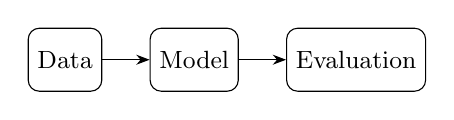
\begin{tikzpicture}[box/.style={draw,rounded corners,minimum height=8mm,align=center,font=\small},node distance=6mm,>={Stealth}]
  \node[box] (data) {Data};
  \node[box,right=of data] (model) {Model};
  \node[box,right=of model] (eval) {Evaluation};
  \draw[->] (data) -- (model);
  \draw[->] (model) -- (eval);
\end{tikzpicture}

  \caption{Method overview.}
  \label{fig:method}
\end{figure}
Describe the setup precisely enough to reproduce it. Figure~\ref{fig:method} shows the method.

\section{Results}
Report every condition with its spread, seed count and tests.

\section{Discussion}
What the results mean, and alternative explanations.

\section{Limitations}
What this can't show.

\section{Conclusion}
What was found, and what should come next.

\nocite{example}
\bibliographystyle{IEEEtran}
\bibliography{refs}
\end{document}
